\documentclass[11pt,a4paper]{article}

% ---------------------------------------------------------------------------
% Inherited chemical-state selection across serial transfers: a finite
% stochastic construction with a machine-checked proof.
%
% Author metadata: set the macros below before submission.  They are
% deliberately left blank in this version.  \CompanionAuthor is the author
% printed for the companion manuscripts in refs.bib; \RepositoryNote is where
% the public repository location goes.
% ---------------------------------------------------------------------------
\newcommand{\PaperAuthor}{}
\newcommand{\PaperAffiliation}{}
\newcommand{\PaperDate}{15 September 2026}
\newcommand{\CompanionAuthor}{Anonymous}
\newcommand{\RepositoryNote}{The repository location will be supplied with the author information.}

\usepackage[T1]{fontenc}
\usepackage[utf8]{inputenc}
\usepackage{lmodern}
\usepackage{microtype}
\usepackage[a4paper,margin=1.05in]{geometry}
\usepackage{amsmath,amssymb,amsthm,mathtools}
\usepackage{booktabs}
\usepackage{array}
\usepackage{longtable}
\usepackage{enumitem}
\usepackage{xcolor}
\usepackage{graphicx}
\usepackage{tikz}
\usetikzlibrary{arrows.meta,positioning,calc}
\usepackage[obeyspaces,spaces]{url}
\usepackage[numbers,sort&compress]{natbib}
\usepackage[colorlinks=true,linkcolor=blue!55!black,citecolor=blue!55!black,urlcolor=blue!55!black]{hyperref}
\hypersetup{pdftitle={Inherited chemical-state selection across serial transfers: a finite stochastic construction with a machine-checked proof},
  pdfkeywords={chemical inheritance, serial transfer, protocell selection, stochastic reaction networks, sampling without replacement, Lean}}

\DeclareUrlCommand\lean{\urlstyle{tt}}
\setlist{itemsep=2pt,topsep=3pt}
\setlength{\emergencystretch}{1.5em}
\setlength{\LTcapwidth}{\textwidth}
\graphicspath{{figures/}}

\theoremstyle{plain}
\newtheorem{theorem}{Theorem}[section]
\newtheorem{proposition}[theorem]{Proposition}
\newtheorem{lemma}[theorem]{Lemma}
\newtheorem{corollary}[theorem]{Corollary}
\theoremstyle{definition}
\newtheorem{definition}[theorem]{Definition}
\theoremstyle{remark}
\newtheorem{remark}[theorem]{Remark}

\newcommand{\R}{\mathbb R}
\newcommand{\N}{\mathbb N}
\newcommand{\Prob}{\mathbb P}
\newcommand{\E}{\mathbb E}
\newcommand{\eps}{\varepsilon}
\newcommand{\Hs}{H}
\newcommand{\gen}{\mathcal L}
\newcommand{\Var}{\operatorname{Var}}
\newcommand{\ind}{\mathbf 1}
\newcommand{\lo}{\mathrm L}
\newcommand{\hi}{\mathrm H}
\newcommand{\fail}{\bot}

\title{Inherited chemical-state selection across serial transfers:\\[4pt]
\large a finite stochastic construction with a machine-checked proof}
\author{\PaperAuthor\\ \small \PaperAffiliation}
\date{\PaperDate}

\begin{document}
\maketitle

\begin{abstract}
A heritable chemical difference between compartments supports repeated selection only if the selected state survives the operations that separate one competition from the next: growth on a shared resource, transfer of a random subset of intact compartments, a recovery interval without growth, and replenishment. We construct a finite stochastic chemical population in which these operations are specified literally and prove a joint probability guarantee across two complete cycles. The resident chemistry is a four-species count network with thirteen channels, completed to six materially balanced reversible pairs with maintained reservoir activities and a single compatible potential assignment. A shared growth precursor couples all compartments; division is complementary at doubled size; transfer chooses exactly $M$ intact compartments uniformly without replacement, with no dependence on their chemical state; a fixed precursor-free interval returns the very compartments that were selected to a certified ready region; refill supplies fresh precursor in proportion to their actual total size. For a balanced newborn population of $M$ compartments, half in each of two stationary chemical states, we prove that after two cycles both measured chemical types remain present and the high-to-low compartment-count log odds have increased by more than $G_2=\frac75\log2-\frac{19}{250}-2\log\frac{51}{49}=0.814395\ldots$, with certified probability at least $495999/500000$ for the witness $N=6.5536\times10^{22}$ size units and $M=4\times10^{9}$ retained compartments; the high-state fraction consequently exceeds $0.693045\ldots$. The proof combines source-specific exponential barriers for the batch, a second-moment bound for uniform sampling without replacement whose variance is at most its mean, a fixed-time recovery estimate applied to the actual selected compartments, capped service counters that leave the physical law unchanged, and conditional composition of finite stopped laws without any independence assumption. An endpoint identity converts size selection into count selection while charging the division-phase penalty only once at the two endpoints rather than at every cycle. The finite marked laws, all probability inequalities, the source instantiation and the quantitative witnesses are verified in Lean~4. The construction assumes maintained resident activities and effective growth and division; its scale is an existence witness, not a laboratory prediction, and every limitation of scope is stated.
\end{abstract}

\section{Introduction}\label{sec:intro}

Selection in a population of chemical compartments is usually demonstrated through serial transfer: a fraction of a grown culture is diluted into fresh medium, regrows, and is transferred again, and a lineage is called selected when its share of the population increases across transfers~\citep{mills1967,lincoln2009}. For compartments whose heritable difference is a chemical composition rather than a template sequence, three separate things must hold for this protocol to select. The composition must change reproductive output while the compartments compete for a shared resource~\citep{chen2004,adamala2013,lu2024,zwicker2017}. The composition must be copied into every descendant through growth, dilution and random partition of finitely many molecules~\citep{segre2000,vasas2010,virgo2015}. And the composition must survive the interventions between competitions: the random removal of most of the population at transfer, the interval in which the retained compartments sit without growth, and the refill that starts the next competition. A theorem about one batch of competition~\citep{batch2026} does not settle the third point, because the compartments alive at the end of a batch have arbitrary division phases and arbitrary positions inside the certified chemical region, and nothing forces the ones that happen to be retained to be prepared for another batch.

This paper proves a joint guarantee for one explicit stochastic model across two complete transfer cycles. The population is a finite count reaction network coupled through one shared precursor pool, with complementary division at doubled size and a certified chemical readout. The operations of a cycle, batch growth to a nutrient endpoint, uniform selection of exactly $M$ intact compartments, a precursor-free recovery interval and proportional refill, are specified as literal transition rules, and every probability is computed under one finite stopped law per stage composed conditionally. The statement is about the number of retained compartments of each measured chemical type at the end of the second cycle, compared with the balanced newborn founders. It carries explicit error terms for every stage and it makes no independence assumption between compartments, between stages, or between cycles.

\paragraph{Relation to prior work.}
Compositional heredity in assemblies and autocatalytic networks has been analysed since \citet{segre2000} and \citet{szathmary1987}, together with sharp doubts about its evolvability~\citep{vasas2010,vasas2012}; \citet{nowak2008} study selection in prelife dynamics, and \citet{matsubara2026} give conditions for Darwinian evolution in compartmentalized autocatalytic networks, including a Moran-type population~\citep{moran1958} with division at doubled volume and random removal. Experimental RNA networks show trade-offs between reproduction, variation and compositional persistence~\citep{ameta2021}, and the general programme is framed by the theory of autocatalytic sets~\citep{kauffman1986,hordijk2004,blokhuis2020,nghe2015}. The distinction between a system that reproduces once and one that can be maintained through repeated dilution is central to the theory of replicators and reproducers~\citep{eigen1971,szathmary2006}, and its mathematical setting is a hybrid system of a continuous competition between transfers and an instantaneous map at each transfer, as in continuous-culture theory~\citep{smithwaltman1995}. That asynchronously dividing lineages can differ in material without differing in number is a classical observation~\citep{powell1956,taheri2015} and is the reason our result is stated in compartment counts. The resident network is taken unchanged from an earlier chemical-copying study~\citep{copying2026}, and finite-count inheritance under bounded food supplies is treated in~\citep{inheritance2026}; the materially balanced completion follows the method of~\citep{thermo2026}; the batch estimates extend the single-batch theorem of~\citep{batch2026}; and a deterministic companion~\citep{recovery2026} proves repeated harvesting for a reversible autocatalytic reactor under interventions that depend on the state. None of these works proves a finite-count probability theorem across transfer, recovery and refill with the outcome measured in compartment counts; that is the contribution here. We make no priority claim on chemically driven compartment competition, on complementary division, or on the serial-transfer protocol itself.

\paragraph{Contributions.}
\begin{enumerate}[label=(\roman*)]
\item \emph{A two-cycle law with explicit error} (Theorem~\ref{thm:law}). For every newborn size $N\ge1.4\times10^{20}$, every even number $M$ of founders, every growth coefficient $0<\gamma\le10^{-11}$ and every finite service quota, the successful output of two complete cycles, with both measured types present and count log odds increased by more than $G_2$, has probability at least $1-\delta(1/2)-\delta(1/100)$, where the per-cycle error $\delta(p)$ in \eqref{eq:delta} is an explicit function of $N$, $M$, $\gamma$, the count floor $p$ and the quotas.
\item \emph{Certified witnesses} (Theorem~\ref{thm:witness}). Two complete source instances are closed by exact rational arithmetic: $N=6.5536\times10^{22}$, $M=4\times10^{9}$ with confidence $495999/500000$, and $N=1.31072\times10^{23}$, $M=10^{15}$ with confidence $497999/500000$. The certified log-odds threshold is the exact expression $G_2$, not a rounded decimal.
\item \emph{Mechanism.} Four ingredients carry the argument. Ancestral size totals are conserved by complementary division and grow at rates sandwiched by the certified $z$ concentrations, which makes a normalized exponential of a logarithmic combination a drift barrier for the size odds (Section~\ref{sec:batch}). Uniform sampling without replacement has nonpositive inclusion covariances, so the variance of a weighted retained total is at most its mean and a Chebyshev bound with a $1/M$ tail suffices (Section~\ref{sec:transfer}). Recovery at zero precursor acts on the selected compartments themselves, whose sizes are frozen, and the same quadratic energy that certifies the batch certifies their return (Section~\ref{sec:recovery}). Service counters that saturate without stopping the physical source give quota bounds with the marginal law unchanged (Section~\ref{sec:service}).
\item \emph{Endpoint phase correction} (Lemma~\ref{lem:phase}). Log count odds equal log size odds minus a mean-size phase bounded by $\log2$. The phase telescopes across cycles, so $K$ cycles pay the phase penalty only at the two endpoints, and newborn founders pay it once. Without this identity each cycle would lose $2\log2$, more than its certified gain.
\item \emph{Operational accounting} (Section~\ref{sec:budgets}). Explicit uniform clocks, explicit quotas, a hard expenditure cutoff that agrees with the maintained model on every event word within budget, separate material accounts for precursor, retained and discarded cells, residual medium and reservoir exchange, and the elapsed model time.
\item \emph{Verification.} The finite stopped laws, every probability inequality, the source certificates, the conditional composition, the count conversion and the two witnesses are verified in Lean~4~\citep{demoura2021} with Mathlib~\citep{mathlib2020}; Appendix~\ref{app:formal} maps each claim to its declaration. An exact replay script re-derives every constant printed here.
\end{enumerate}

\paragraph{Three kinds of evidence.}
Machine-checked statements, conventional proofs, and numerical diagnostics are kept apart throughout. The finite marked laws, the source-specific barrier inequalities, the transfer, recovery, service and composition bounds, the count conversion and the exact witnesses are Lean-verified. The identification of the finite stopped laws with a continuous-time population, the population summation behind the explicit clock values, and the decimal conversions of exact thresholds are conventional and are labelled as such. The figure and the term-by-term error table of Section~\ref{sec:numbers} evaluate proved formulas at high precision; they prove nothing and simulate nothing.

\paragraph{What is not claimed.}
The resident reservoir species are maintained at unit activity by external supply, and their finite gross-exchange allowances are counts of exchanged molecules, not a model of autonomous depletion and not a free-energy accounting~\citep{polettini2014,rao2016}. Growth and division are effective constitutive rules; no membrane mechanics is derived. Two cycles are certified; the same eligibility estimate does not certify a third start at the stated floors, and no indefinite coexistence, fixation probability or evolutionary innovation is asserted. The witness sizes are astronomically large because every certificate is conservative; the theorem is an existence statement about a specified effective model, not a laboratory prediction, and Section~\ref{sec:discussion} lists what an experimental application would first have to identify.

\paragraph{Organization.}
Section~\ref{sec:model} specifies the chemistry, the operations and the analytical marks. Section~\ref{sec:main} states the results. Section~\ref{sec:tools} collects the finite-law tools. Sections~\ref{sec:batch}--\ref{sec:count} prove the theorems stage by stage. Section~\ref{sec:consequences} derives measurable consequences, Section~\ref{sec:budgets} the operational accounting, Section~\ref{sec:numbers} the quantitative evaluation and its conservatism, and Section~\ref{sec:discussion} the scope and open questions. Appendix~\ref{app:source} contains the source certificate, Appendix~\ref{app:barriers} the barrier forms, and Appendix~\ref{app:formal} the formal source map and reproduction commands.

\section{The chemical source and the operating protocol}\label{sec:model}

\subsection{Resident channels and their material completion}\label{sec:chemistry}
A compartment, called a cell below, has an integer size $m\in\N$ and internal counts $n=(n_A,n_B,n_z,n_\Hs)\in\N^4$; its concentration vector is $x=n/m$. The newborn size is $N$, and a live cell has $N\le m<2N$ between divisions. The thirteen resident channels are the two directions of the first six rows of Table~\ref{tab:source} followed by its last row. Every propensity is a literal count propensity with falling-factorial factors for identical reactants; it vanishes when a reactant is absent. No fitness parameter is assigned: the only difference between chemical states that matters for growth is their resident concentration of the growth-linked species $z$.

\begin{table}[tb]
\centering\small
\caption{The resident count source. $F$, $G$, $R_A$ and $R_B$ are reservoir species maintained at unit activity; $W_\Hs$ collects the sink. The thirteen channels are the two directions of the six reversible pairs and the irreversible last row.}
\label{tab:source}
\begin{tabular}{clll}
\toprule
Pair & Reaction & Forward propensity & Reverse propensity\\
\midrule
1 & $A\rightleftharpoons B+z$ & $n_A$ & $n_Bn_z/m$\\
2 & $z+F\rightleftharpoons \Hs$ & $16n_z$ & $n_\Hs$\\
3 & $\Hs\rightleftharpoons 2z$ & $n_\Hs$ & $2n_z(n_z-1)/m$\\
4 & $R_A\rightleftharpoons A$ & $6m$ & $n_A$\\
5 & $R_B\rightleftharpoons B$ & $27m$ & $n_B$\\
6 & $B+G\rightleftharpoons 2A$ & $10^{-5}n_B$ & $10^{-5}n_A(n_A-1)/m$\\
--- & $\Hs\longrightarrow W_\Hs$ & $10^{-4}n_\Hs$ & ---\\
\bottomrule
\end{tabular}
\end{table}

The four internal species alone cannot be mass-balanced: pair~3 forces a formal mass $m_\Hs=2m_z$ while the pair $z\rightleftharpoons\Hs$ of the original open-system table would force $m_\Hs=m_z$. The completion of Table~\ref{tab:source} resolves this with the reservoir species. Assigning the formal elemental weights
\begin{equation}\label{eq:element}
(A,B,z,\Hs,F,G,R_A,R_B,W_\Hs)\mapsto(2,1,1,2,1,3,2,1,2)
\end{equation}
balances every displayed reaction, and the dimensionless potentials
\begin{equation}\label{eq:potential}
(\mu_A,\mu_B,\mu_z,\mu_\Hs,\mu_F,\mu_G,\mu_{R_A},\mu_{R_B},\mu_{W_\Hs})=(0,0,0,-\log2,\,3\log2,\,0,\,\log6,\,\log27,\,0)
\end{equation}
reproduce every forward-to-reverse rate ratio of the six pairs through $\log(k_+/k_-)=\sum(\text{reactant}-\text{product})\,\mu$. At unit reservoir activities the maintained propensities coincide channel by channel with the count propensities of the earlier open-system table~\citep{copying2026,batch2026}, so every estimate proved for that table applies unchanged. The balanced completion concerns the resident network; growth and division are the effective constitutive rules specified next, and the reservoirs are maintained externally for the finite duration of the protocol (Section~\ref{sec:budgets}).

\subsection{Shared precursor, growth and complementary division}\label{sec:growth}
Let $Q\in\N$ be a shared precursor stock and $\Omega$ its initial value in a batch. Each cell grows with propensity
\begin{equation}\label{eq:growth}
\gamma\,\frac{Q}{\Omega}\,n_z ,
\end{equation}
which vanishes when $Q=0$ or $n_z=0$. A growth event consumes one unit of $Q$ and one internal $z$ and increases $m$ by one; the two are retained as one unit of size material. If the resulting size is $2N$, the same event replaces the parent by two daughters of size $N$: for each internal species, one daughter receives a $\operatorname{Binomial}(n_i,1/2)$ count and the other the complement, independently across species. The daughters are complementary, not independent, and they inherit the parent's analytical ancestry tag, which enters no propensity and no draw. Division is processed even when the triggering growth event is the one that reaches the batch endpoint. The parameter $\gamma$ has units of inverse time once the unit of $Q/\Omega$ is fixed; the theorem assumes $0<\gamma\le10^{-11}$ in the time unit of Table~\ref{tab:source}, that is, growth is slow compared with resident chemistry.

\subsection{Stationary compositions, readiness and readout}\label{sec:ready}
The density-limit drift of the resident channels (Appendix~\ref{app:source}) has stationary compositions $s_\lo$ and $s_\hi$ whose $z$ coordinates lie in the exact rational intervals
\begin{equation}\label{eq:roots}
z_\lo\in[0.99579401232,\,0.99579401233],\qquad z_\hi\in[2.97636724376,\,2.97636724377];
\end{equation}
the other coordinates are rational functions of $z$ given there. These are stationary points of the zero-growth density drift; nothing is claimed about stationary point masses of the finite count chain. Let $E_i(x-s_i)$, $i\in\{\lo,\hi\}$, be the positive definite quadratic forms of Appendix~\ref{app:source}, and put
\begin{equation}\label{eq:constants}
a=\frac1{512\,000\,000},\qquad \alpha=10^{-12},\qquad u=N\alpha a .
\end{equation}
A cell of analytical type $i$ is \emph{ready} when $E_i\le a$ and $N\le m<2N$; a \emph{ready population} consists of exactly $M$ ready cells. At a census a cell is classified as \emph{high} if its actual concentration $n_z/m$ exceeds $2$ and as \emph{low} otherwise; $C_\hi$ and $C_\lo$ denote these measured counts. On the ready region the readout agrees with the analytical tag (Section~\ref{sec:consequences} gives the explicit separation), so on the successful event ancestry counts are measured chemical counts.

\subsection{One operating cycle}\label{sec:cycle}
Given a ready population of total size $W_0=\sum_jm_j$, one cycle consists of the following operations (Figure~\ref{fig:protocol}).
\begin{enumerate}
\item \emph{Batch.} Supply fresh precursor $Q=\Omega=4W_0$ and run the shared-source population until $Q=W_0$, subject to the deadline $T=8/\gamma$.
\item \emph{Transfer.} At the endpoint, choose exactly $M$ intact cells uniformly without replacement among all live cells. Record every other cell as discarded and remove the residual precursor medium.
\item \emph{Recovery.} Keep the selected cells, with their current sizes and counts, at $Q=0$ for $5376$ time units. Resident chemistry continues; growth and division cease.
\item \emph{Refill.} Supply $Q=\Omega=4\sum_jm_j$ for the retained cells. On success this is the next ready population.
\end{enumerate}
Recovery does not replace the selected cells by fresh samples from any equilibrium: the internal chemistry of each selected cell evolves under its resident source while its size and ancestry stay fixed. No operation reads a tag or a chemical state; the transfer law assigns equal mass to every $M$-subset, and refill depends only on the sizes.

\begin{figure}[tb]
\centering
\resizebox{\linewidth}{!}{%
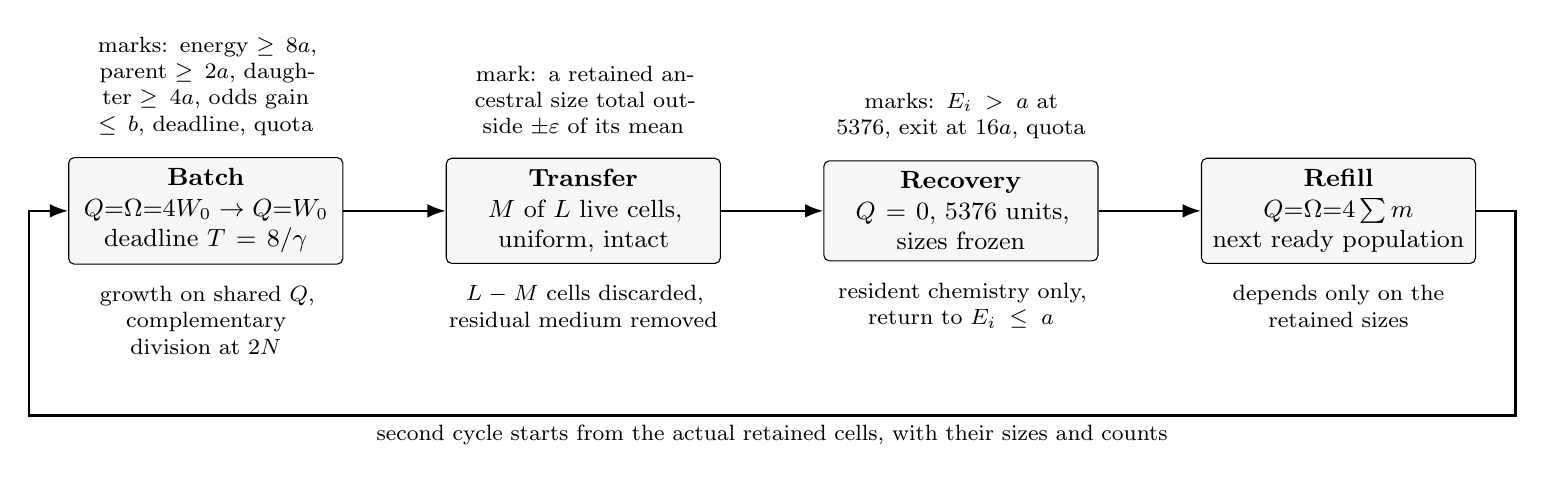
\begin{tikzpicture}[>=Latex,font=\small,
  box/.style={draw,rounded corners=2pt,align=center,minimum height=1.15cm,inner sep=4pt,fill=black!3,text width=3.2cm},
  lab/.style={font=\footnotesize,align=center,text width=3.6cm}]
\node[box] (batch) {\textbf{Batch}\\ $Q{=}\Omega{=}4W_0\to Q{=}W_0$\\ deadline $T=8/\gamma$};
\node[box,right=1.3cm of batch] (transfer) {\textbf{Transfer}\\ $M$ of $L$ live cells,\\ uniform, intact};
\node[box,right=1.3cm of transfer] (recovery) {\textbf{Recovery}\\ $Q=0$, $5376$ units,\\ sizes frozen};
\node[box,right=1.3cm of recovery] (refill) {\textbf{Refill}\\ $Q{=}\Omega{=}4\sum m$\\ next ready population};
\draw[->,thick] (batch) -- (transfer);
\draw[->,thick] (transfer) -- (recovery);
\draw[->,thick] (recovery) -- (refill);
\coordinate (br) at ($(refill.east)+(0.5,0)$);
\coordinate (bl) at ($(batch.west)+(-0.5,0)$);
\draw[->,thick] (refill.east) -- (br) -- ($(br)+(0,-2.6)$) -- ($(bl)+(0,-2.6)$) -- (bl) -- (batch.west);
\node[font=\footnotesize,below] at ($(br)!0.5!(bl)+(0,-2.6)$) {second cycle starts from the actual retained cells, with their sizes and counts};
\node[lab,below=0.15cm of batch] {growth on shared $Q$,\\ complementary division at $2N$};
\node[lab,below=0.15cm of transfer] {$L-M$ cells discarded,\\ residual medium removed};
\node[lab,below=0.15cm of recovery] {resident chemistry only,\\ return to $E_i\le a$};
\node[lab,below=0.15cm of refill] {depends only on the\\ retained sizes};
\node[lab,above=0.15cm of batch] {marks: energy $\ge8a$, parent $\ge2a$, daughter $\ge4a$, odds gain $\le b$, deadline, quota};
\node[lab,above=0.15cm of transfer] {mark: a retained ancestral size total outside $\pm\eps$ of its mean};
\node[lab,above=0.15cm of recovery] {marks: $E_i>a$ at $5376$, exit at $16a$, quota};
\end{tikzpicture}}
\caption{One operating cycle and the analytical marks that define the failure quotient. The marks are used only to bound probabilities; no operation of the protocol reads them.}
\label{fig:protocol}
\end{figure}

\subsection{Analytical marks and the failure quotient}\label{sec:marks}
For the analysis, a trajectory is marked as failed when it leaves a certified chemical region, when a division parent or daughter is outside its admitted region, when the batch misses its nutrient endpoint by the deadline, when the batch size-odds gain falls short of its target, when a retained ancestral size total leaves its tolerance, when a selected cell has not returned to readiness after recovery, or when a service counter saturates. Each stage is a finite marked jump model stopped at its first mark or at its physical endpoint, and the stopped record keeps the physical transition that triggered the stop. The output of a stage is either the actual physical population or a single failure symbol $\fail$, which is absorbing. Failure mass is never renormalized, no successful trajectory is resampled, and no mark licenses an intervention: the operations of Section~\ref{sec:cycle} are the same for every trajectory. Section~\ref{sec:localization} explains how these finite stopped laws are read as an ongoing population process.

\section{Main results}\label{sec:main}

Set
\begin{equation}\label{eq:gain}
b=\frac35\log4-\frac{19}{500},\qquad \ell=\log\frac{51}{49},\qquad g=b-\ell,\qquad G_2=2g-\log2=\frac75\log2-\frac{19}{250}-2\log\frac{51}{49}.
\end{equation}
Here $b$ is the certified size-odds gain of one batch, $\ell$ the size-odds loss allowed at transfer for tolerance $\eps=1/50$, $g$ the certified size-odds gain of one cycle, and $G_2$ the two-cycle count-odds gain for newborn founders after the single endpoint phase penalty $\log2$ of Lemma~\ref{lem:phase}. For $N$, $M$, quotas $J_B,J_R\ge1$, clock bounds $q_B,q_R$, a count floor $p\in(0,1]$ and $\eps=1/50$, the per-cycle error is
\begin{align}\label{eq:delta}
\delta(p)={}&A(N,M,T)+e^{-N/2500}+e^{-19N/500000}+\frac{Tq_B}{J_B}
 +\frac{32}{\eps^2pM}+M\Bigl(R(u)+\frac{5376\,q_R}{J_R}\Bigr),
\end{align}
where the batch chemical error $A(N,M,T)$ is given in \eqref{eq:A} and the single-cell recovery error $R(u)$ in \eqref{eq:R}. The first four terms belong to the batch (chemistry, deadline, size odds, service), the fifth to the transfer, and the last to recovery of the $M$ selected cells (return and service).

\begin{theorem}[Two-cycle law for balanced newborn founders]\label{thm:law}
Let $N\ge1.4\times10^{20}$, let $M=2K$ with $K\ge1$, let $0<\gamma\le10^{-11}$ and $T=8/\gamma$. Let $q_B$ and $q_R$ be finite clock bounds dominating every rate of the batch and recovery source models, with $q_R\ge u/672$ and $q_B\ge9N\gamma/40000$, and let $J_B,J_R\ge1$. Then there exist stationary compositions with $z$ coordinates in \eqref{eq:roots} and a balanced ready population $s$ of $K$ low and $K$ high newborn cells, all of size $N$, whose readout agrees with their tags. Under the two-cycle law started from $s$, the event that the output is a physical population with both measured counts positive and
\begin{equation}\label{eq:main}
\log\frac{C_\hi(2)}{C_\lo(2)}-\log\frac{C_\hi(0)}{C_\lo(0)}>G_2
\end{equation}
has probability at least $1-\delta(1/2)-\delta(1/100)$. On that event the final population is ready for the same refill rule.
\end{theorem}

\begin{theorem}[Certified witnesses]\label{thm:witness}
For $\gamma=10^{-11}$, $T=8\times10^{11}$ and finite quotas satisfying $Tq_B/J_B<10^{-3}$ and $M\cdot5376\,q_R/J_R<10^{-3}$, which exist for every admissible clock bound, the conclusion of Theorem~\ref{thm:law} holds with the following confidences. For $N=65536\times10^{18}$ and $M=4\times10^{9}$,
\[
\Prob\{\text{success and \eqref{eq:main}}\}\ \ge\ \frac{495999}{500000}=0.991998;
\]
for $N=131072\times10^{18}$ and $M=10^{15}$,
\[
\Prob\{\text{success and \eqref{eq:main}}\}\ \ge\ \frac{497999}{500000}=0.995998 .
\]
In both cases $C_\hi(0)=C_\lo(0)=M/2$, $G_2>0.8143953$ and $C_\hi(2)/M>0.6930453$.
\end{theorem}

The successful event of both theorems is the output with both positive measured counts and \eqref{eq:main}; its probability is bounded below by that of the stronger joint event that every constituent stage succeeds. The two-cycle statement gives cumulative enrichment across two cycles; it does not assert that the count ratio increases between every pair of consecutive censuses. Nothing in the hypotheses assumes a successful return kernel, independent cells, independent service counters, or a successful selection: all failure mass remains in the law. The smaller witness reduces $NM$ by a factor $500000$ relative to the original one; the price is the transfer term $32/(\eps^2pM)$, which is $0.002$ at $p=1/100$ and dominates its error budget.

\begin{corollary}[Fractions and one cycle]\label{cor:fraction}
For the balanced start, \eqref{eq:main} is equivalent to $f_\hi(2)>e^{G_2}/(1+e^{G_2})=0.693045342\ldots$. On the successful first cycle alone the newborn phase correction gives
\[
\log\frac{C_\hi(1)}{C_\lo(1)}-\log\frac{C_\hi(0)}{C_\lo(0)}>g-\log2=0.06062410149\ldots,\qquad f_\hi(1)>0.515151385\ldots .
\]
The elementary bounds $\log2\ge\frac12$ and $\log\frac{51}{49}\le\frac2{49}$ give the rational thresholds $519/24500$ after one cycle and $3322/6125$ after two; the logarithmic thresholds are stronger and are the certified ones.
\end{corollary}

\begin{remark}[The original root theorem]\label{rem:root}
The first compiled form of the result, \lean{source_serial_transfer_c3}, states the original witness with confidence $99/100$ and the count-odds threshold $519/12250=0.04236\ldots$, obtained from $2g-2\log2$ by charging the phase penalty at both endpoints and using only the rational bounds. It also carries a protocol certificate (Section~\ref{sec:budgets}) bundling the material balance, the potential assignment, type-neutral sampling and refill, the discard identity and the quota material bounds. Theorems~\ref{thm:law} and \ref{thm:witness} strengthen it by the newborn phase identity, the exact logarithmic threshold and the sharper exact error certificates; the original declaration is unchanged.
\end{remark}

\section{Finite laws and comparison tools}\label{sec:tools}

\subsection{Uniformized marked laws}
A finite marked jump model consists of a finite state set $S$, channels $r$ with nonnegative rates $a_r(x)$ and transitions $F_r(x)\in S$, and terminal states with zero total rate. For a clock bound $q\ge\sup_x\sum_ra_r(x)$, $q>0$, the uniformized kernel~\citep{jensen1953} is
\begin{equation}\label{eq:kernel}
P(x,y)=\Bigl(1-\frac{\sum_ra_r(x)}q\Bigr)\ind_{y=x}+\sum_r\frac{a_r(x)}q\ind_{F_r(x)=y},
\end{equation}
and the time-$t$ law is the Poisson mixture
\begin{equation}\label{eq:poisson}
P_t=e^{-qt}\sum_{j\ge0}\frac{(qt)^j}{j!}P^j .
\end{equation}
Channels that leave the physical state unchanged keep their marks; the virtual holds of uniformization carry no mark and spend no service. Because $S$ is finite, \eqref{eq:poisson} is a probability law on $S$, and the generator $\gen V(x)=\sum_ra_r(x)(V(F_r(x))-V(x))$ satisfies $\gen V=q(PV-V)$. Killing is represented by a failure state at which every observable used below vanishes; absorbing terminal records preserve the actual stopped output. The stopped laws of the batch, recovery and service stages are of this form; the transfer law is the uniform law on $M$-subsets. The statements of Section~\ref{sec:main} refer to the compositions of these finite laws, which is what is machine-checked.

\subsection{Comparison inequalities}
The following elementary inequalities are the only probability tools needed; they are the finite-law form of Foster--Lyapunov comparison arguments~\citep{meyntweedie1993,gupta2014,kuntz2019}, proved by iterating the one-step inequality for $P$ and summing \eqref{eq:poisson}.

\begin{lemma}[Drift barrier]\label{lem:barrier}
Let $V\ge0$ satisfy $\gen V\le d$ on $S$. Then $\E V(X_t)\le V(X_0)+dt$. If moreover $V\ge H_*>0$ on an absorbing set $A$, then $\Prob\{X_t\in A\}\le(V(X_0)+dt)/H_*$; for $d\le0$ the bound is $V(X_0)/H_*$.
\end{lemma}

\begin{lemma}[Affine relaxation]\label{lem:affine}
Let $V\ge0$ satisfy $\gen V\le-kV+c$ with $0<k\le q$. Then $\E V(X_t)\le e^{-kt}V(X_0)+(c/k)(1-e^{-kt})\le e^{-kt}V(X_0)+c/k$.
\end{lemma}

\begin{proof}
The one-step inequality is $PV\le(1-k/q)V+c/q$ with $1-k/q\in[0,1)$, hence $P^jV\le(1-k/q)^jV+(c/k)(1-(1-k/q)^j)$, and $\sum_je^{-qt}(qt)^j(1-k/q)^j/j!=e^{-kt}$.
\end{proof}

\begin{lemma}[Killed observable]\label{lem:killed}
Let $V\ge0$ vanish on terminal states and satisfy $\gen V\le-kV$ on active states with $0\le k\le q$. Then $\E V(X_t)\le e^{-kt}V(X_0)$. If $V\ge H_*>0$ on every active state, the probability of still being active at time $t$ is at most $e^{-kt}V(X_0)/H_*$.
\end{lemma}

\begin{lemma}[Cover and union]\label{lem:union}
If the failure set of a stopped law is contained in a finite union of sets $A_1,\dots,A_r$, then the success probability is at least $1-\sum_i\Prob(A_i)$.
\end{lemma}

\subsection{Failure quotient and conditional composition}\label{sec:composition}
Let $\mu$ be a finite law on $S$ and $A\subseteq S$ a success set with a map $f:A\to S'$ to the physical output. The \emph{guarded push} of $\mu$ is the law on $S'\cup\{\fail\}$ that sends $x\in A$ to $f(x)$ and every $x\notin A$ to $\fail$. It has the same mass on the success outputs as $\mu$ has on $A$; nothing is conditioned or resampled. Stages are composed by binding: if $\mu$ is the law of one stage and $\kappa_y$ the law of the next stage started from output $y$, with $\kappa_\fail=\delta_\fail$, the composed law is $\mu\kappa$.

\begin{lemma}[Conditional composition]\label{lem:compose}
Suppose $\mu\{A\}\ge1-\delta_1$ and, for every $y\in f(A)$, $\kappa_y\{B_y\}\ge1-\delta_2$ with $B_y$ contained in a target set $C$. Then $\mu\kappa\{C\}\ge1-\delta_1-\delta_2$.
\end{lemma}

\begin{proof}
$\mu\kappa\{C\}\ge\sum_{x\in A}\mu(x)\kappa_{f(x)}\{B_{f(x)}\}\ge(1-\delta_2)\mu\{A\}\ge1-\delta_1-\delta_2$.
\end{proof}

The lemma is applied with stage estimates that are \emph{uniform} over their admitted starting states; that uniformity is what allows them to be used conditionally on any successful past, without independence between stages and without any assumption about the joint law of the sampled and unsampled cells.

\section{The source batch}\label{sec:batch}

\subsection{Preparation and conservation}
\begin{lemma}[Ready founders]\label{lem:founders}
For $N\ge10^{12}$ and every size $N\le m<2N$, rounding the coordinates of $ms_i$ down to integers gives a ready cell of type $i$. Replicating one such low cell and one such high cell $K$ times gives a balanced ready newborn population of $M=2K$ cells of size $N$ whose readout agrees with their tags.
\end{lemma}

\begin{proof}
Each concentration coordinate of the rounded cell differs from $s_i$ by at most $1/m$, so by the upper bound of Appendix~\ref{app:source}, $E_i\le42\|x-s_i\|^2\le168/m^2\le a$ for $m\ge10^{12}$. The coordinates are nonnegative and inside the source box. Readout agreement is the separation of Section~\ref{sec:consequences}. The construction is explicit; no enumeration of a population of $M$ cells is performed.
\end{proof}

\begin{lemma}[Conservation and caps]\label{lem:conservation}
During a batch started from total size $W_0$, growth and complementary division conserve $Q+W=5W_0$ with $W=\sum_jm_j$; at the endpoint $Q=W_0$ one has $W=4W_0$. If the batch starts from $M$ ready cells then $W_0\le2NM$, so throughout the batch $W\le8NM$, there are at most $8M$ live cells, and at most $7M$ divisions occur.
\end{lemma}

\begin{proof}
A growth event moves one unit from $Q$ to $W$ whether or not it divides the parent; a resident event changes no size; complementary division preserves the total size. Every live cell has size at least $N$, so $W\le8NM$ caps the cell count by $8M$ and hence the number of divisions, each of which adds one cell, by $7M$.
\end{proof}

\begin{remark}
The caps allow arbitrary division phases at the start of a batch, which the second cycle requires. The newborn-only cap $4M$ of~\citep{batch2026} is false for such starts: with $N=2$ and a single founder of size $3$, the endpoint $W=12$ can be reached by the configuration $(2,2,2,3,3)$ of five cells. This small exact counterexample was found before the population bounds were proved, and it fixed the caps used here.
\end{remark}

\subsection{Local chemical certificate}
For each type, the quadratic energy $E_i$ satisfies $\|y\|^2/200\le E_i(y)\le42\|y\|^2$, and on the outer region $E_i<16a$ every coordinate error is at most $1/400$. The source-specific generator estimate below is the local chemical input to all population bounds; its derivation is in Appendix~\ref{app:source}.

\begin{lemma}[Local dissipation]\label{lem:local}
For $N\ge1.4\times10^{20}$, $0\le\gamma'\le10^{-11}$ and $m\ge N$, on the region $E_i<16a$,
\begin{equation}\label{eq:local}
\gen_{\gamma'}\,e^{N\alpha E_i}\le-\frac u{672}\,e^{N\alpha E_i}+\frac u{672}\,2e^{u/2},
\end{equation}
where $\gen_{\gamma'}$ is the generator of the thirteen resident channels together with the size-diluting growth jump of coefficient $\gamma'$, including the finite-count falling-factorial corrections.
\end{lemma}

In a batch, $\gamma'=\gamma Q/\Omega\le\gamma$; in recovery, $\gamma'=0$.

\subsection{Chemical failures during the batch}
Three kinds of chemical failure are marked: an \emph{outer} failure when a live cell reaches $E_i\ge8a$; a \emph{division-parent} failure when a cell divides with $E_i\ge2a$; and a \emph{partition} failure when a daughter of an admitted parent has $E_i\ge4a$. The finite active domain is preserved by every positive-rate transition, so no unmarked exit occurs.

\begin{proposition}[Batch chemical error]\label{prop:chem}
Under the hypotheses of Lemma~\ref{lem:local}, for a batch started from $M$ ready cells, the probability of any chemical failure before or at the nutrient endpoint is at most
\begin{align}\label{eq:A}
A(N,M,T)={}&Me^{-7u}+14Me^{-4u}+\frac{MTu}{42}e^{-15u/2}+Me^{-u}+\frac{MTu}{42}e^{-3u/2}\nonumber\\
&+56M\exp\Bigl(-\frac N{35\cdot10^{12}}\Bigr).
\end{align}
On the complementary event every cell alive at the endpoint has $E_i<8a$.
\end{proposition}

\begin{proof}
Let $V_j=e^{N\alpha E_{i(j)}}$ for live cell $j$ and consider the population observables $\Phi_1=\sum_jV_j$ and $\Phi_2=\sum_je^{\lambda(m_j-2N)}V_j$ with $\lambda=10^{-15}$. By Lemma~\ref{lem:local} and the cap of $8M$ live cells, both have drift at most $8M\cdot\frac u{672}\,2e^{u/2}$ on the unflagged domain, the size factor of $\Phi_2$ being absorbed by the small-growth premise. Initially $\Phi_1,\Phi_2\le Me^u$. A division with admitted parent and daughters adds at most $2e^{4u}$ to $\Phi_1$; for $\Phi_2$ the parent enters with factor $1$ at $m=2N$ and each daughter with factor $e^{-\lambda N}$ at $m=N$, and $2e^{4u-\lambda N}\le1$ for $N\ge1.4\times10^{20}$, so two admitted daughters cost no more than their parent. Lemma~\ref{lem:barrier} with barrier $e^{8u}$ for $\Phi_1$, charging at most $14M$ daughter initializations, bounds the outer failure; with barrier $e^{2u}$ for $\Phi_2$ it bounds the division-parent failure. Conditional on an admitted parent, the complementary binomial partition of counts at most $70N$ perturbs each daughter concentration by more than $10^{-6}$ with probability at most $8e^{-N/(35\cdot10^{12})}$, a Hoeffding bound~\citep{hoeffding1963} over the four species and two daughters, and a smaller perturbation keeps the daughter inside $4a$ since $42\cdot16\cdot10^{-12}<a$; at most $7M$ partitions occur. Summing the three bounds gives the unexpanded form displayed in Appendix~\ref{app:barriers}, whose expansion is \eqref{eq:A} without approximation.
\end{proof}

\subsection{Size odds and deadline}
For a population write $B_\hi$ and $B_\lo$ for the total sizes of the cells of high and low ancestry, $Z_\hi$ and $Z_\lo$ for their total $z$ counts, and $S=\log(B_\hi/B_\lo)$ for the size log odds. Resident events and complementary divisions leave $B_\hi$ and $B_\lo$ unchanged; a growth event increases exactly one of them by one. Within the certified regions the coordinate error at most $1/400$ and the root intervals \eqref{eq:roots} give
\begin{equation}\label{eq:sandwich}
2.97\,B_\hi\le Z_\hi\le3\,B_\hi,\qquad 0.99\,B_\lo\le Z_\lo\le1.01\,B_\lo .
\end{equation}
The growth propensity \eqref{eq:growth} multiplies every $z$ count by the same factor $\gamma Q/\Omega$, so the relative growth advantage of the high ancestry is preserved by the shared resource.

\begin{proposition}[Size-odds barrier]\label{prop:odds}
On the event of no chemical failure, the size log odds at the nutrient endpoint satisfy $S_{\rm end}-S_{\rm start}>b$ except with probability at most $e^{-19N/500000}$; both ancestral size totals stay positive.
\end{proposition}

\begin{proof}
Put $V(H,L)=\exp\bigl(\frac N{1000}[-\log H+\log L+\frac35\log(H+L)]\bigr)$ for $H=B_\hi$, $L=B_\lo$, normalized by its starting value. Its two logarithmic increments $d_H,d_L$ are displayed in Appendix~\ref{app:barriers}, and the scalar inequality $Z_\hi(e^{d_H}-1)+Z_\lo(e^{d_L}-1)\le0$ holds for all $H,L\ge N$, $N\ge1000$, under \eqref{eq:sandwich}; multiplication by the common nonnegative growth coefficient preserves its sign, so $V$ has nonpositive drift. At the endpoint $H+L=4W_0$, and failure of the gain $b$ forces $V/V_0\ge\exp\bigl(\frac N{1000}[\frac35\log4-b]\bigr)=e^{19N/500000}$. Lemma~\ref{lem:barrier} with $V_0/V_0=1$ gives the bound. Positivity of the ancestral totals is preserved by every transition.
\end{proof}

\begin{proposition}[Deadline]\label{prop:deadline}
The probability that the batch has not reached $Q=W_0$ by $T=8/\gamma$ without an earlier chemical failure is at most $e^{-N/2500}$.
\end{proposition}

\begin{proof}
Let $D=\exp\bigl(-\frac N{1000}\log\frac{H+L}{W_0}\bigr)$ on active states and $0$ on terminal ones. Before the endpoint, $Q/\Omega\ge1/4$, so the total growth rate is at least $\gamma\cdot\frac14\cdot0.99(H+L)$ and the generator of $D$ is at most $-\frac{9N\gamma}{40000}D$. Before the endpoint $H+L\le4W_0$, so $D\ge e^{-(N/1000)\log4}$. Lemma~\ref{lem:killed} gives an active probability at $T$ of at most $\exp[-\frac{9N}{5000}+\frac N{1000}\log4]\le e^{-N/2500}$ using $\log4\le7/5$. Early chemical failures are in the chemical cover; a slow batch is therefore not silently excluded by stopping.
\end{proof}

\begin{proposition}[Joint batch estimate]\label{prop:batch}
Let $N\ge1.4\times10^{20}$, $0<\gamma\le10^{-11}$, and let the batch start from $M$ ready cells with both ancestries present. Except with probability at most $A(N,M,T)+e^{-N/2500}+e^{-19N/500000}$, the batch reaches its nutrient endpoint by $T$, every endpoint cell has $E_i<8a$ and lies in $[N,2N)$, both ancestral size totals are positive, and $S_{\rm end}-S_{\rm start}>b$.
\end{proposition}

\begin{proof}
Union of Propositions~\ref{prop:chem}, \ref{prop:odds} and \ref{prop:deadline} under the single batch law (Lemma~\ref{lem:union}); the size bounds are the domain constraints, preserved by every positive-rate transition.
\end{proof}

\section{Uniform transfer of intact cells}\label{sec:transfer}

Condition on the complete batch endpoint: a list of $n$ live cells with sizes $m_j$ and tags, $M\le n\le8M$. The transfer law is uniform on the $\binom nM$ subsets of size $M$; write $I_j$ for the inclusion indicator of cell $j$.

\begin{lemma}[Inclusion moments]\label{lem:moments}
$\E I_j=M/n$ and, for $j\ne k$, $\E I_jI_k=M(M-1)/(n(n-1))\le(M/n)^2$. Hence inclusion covariances are nonpositive.
\end{lemma}

\begin{proof}
Permutation symmetry gives the marginals and pair moments; $M(M-1)/(n(n-1))\le(M/n)^2$ is equivalent to $M\le n$.
\end{proof}

\begin{lemma}[Variance at most mean]\label{lem:variance}
For weights $w_j\in[0,1]$, the retained total $W=\sum_jw_jI_j$ satisfies $\Var W\le\sum_jw_j^2\Var I_j\le\E W$.
\end{lemma}

\begin{proof}
Nonpositive covariances drop the cross terms; $w_j^2\le w_j$ and $\Var I_j\le\E I_j$.
\end{proof}

\begin{proposition}[Uniform transfer]\label{prop:transfer}
Suppose the batch started with each ancestry count at least $pM$ and ended successfully, and let $0<\eps<1$. Except with probability at most
\begin{equation}\label{eq:transfer}
D(p,M,\eps)=\frac{32}{\eps^2pM},
\end{equation}
both retained ancestral size totals lie within relative tolerance $\eps$ of their conditional means, their log ratio differs from the endpoint size log odds by at most $\log\frac{1+\eps}{1-\eps}$, and each retained ancestry count is at least $(1-\eps)pM/16$.
\end{proposition}

\begin{proof}
For one ancestry put $w_j=m_j/(2N)\in[0,1]$ for cells of that ancestry and $w_j=0$ otherwise. The ancestral size total cannot decrease during the batch and starts at least $NpM$, so $\E W=(M/n)\sum_jw_j\ge\frac18\cdot\frac{NpM}{2N}=\frac{pM}{16}$. Chebyshev's inequality with Lemma~\ref{lem:variance} gives $\Prob\{|W-\E W|>\eps\E W\}\le1/(\eps^2\E W)\le16/(\eps^2pM)$, and the union over the two ancestries gives \eqref{eq:transfer}. Both means carry the same factor $M/n$, so their ratio is the endpoint size ratio and the retained log odds lie within $\log\frac{1+\eps}{1-\eps}$ of $S_{\rm end}$. Each retained cell has size below $2N$, so the retained count of an ancestry is at least its retained size total divided by $2N$, which is at least $(1-\eps)\E W\ge(1-\eps)pM/16$. For $n=1$ the sampling is deterministic; in every case considered $n\ge M\ge2$.
\end{proof}

The $1/M$ tail is the price of a second-moment argument. Exponential bounds for sampling without replacement~\citep{hoeffding1963,bardenet2015} would sharpen it, but the second-moment route needs only the nonpositive covariances and a mean floor, and it is what closes the witnesses; Section~\ref{sec:numbers} shows exactly how much it costs.

\section{Recovery of the selected cells}\label{sec:recovery}

\begin{lemma}[Frozen size]\label{lem:frozen}
At $Q=0$ the growth propensity \eqref{eq:growth} vanishes, so a selected cell neither grows nor divides during recovery; its size, its tag and hence both ancestral size totals and counts are unchanged by recovery and by refill.
\end{lemma}

\begin{proposition}[Single-cell return]\label{prop:return}
Start a selected cell with $N\le m<2N$ and $E_i\le8a$ at $Q=0$. After $5376$ time units, the probability that it is not ready, or that it has left the outer region $E_i<16a$ at any time, is at most
\begin{equation}\label{eq:R}
R(u)=e^{-u}+2e^{-u/2}+e^{-8u}+16u\,e^{-31u/2}.
\end{equation}
\end{proposition}

\begin{proof}
Apply Lemma~\ref{lem:affine} to $V=e^{N\alpha E_i}$ with $k=u/672$ and $c=\frac u{672}2e^{u/2}$ from Lemma~\ref{lem:local} at $\gamma'=0$: since $k\cdot5376=8u$ and $V_0\le e^{8u}$, $\E V_{5376}\le1+2e^{u/2}$, and Markov's inequality at level $e^u$ bounds the terminal unready probability by $e^{-u}+2e^{-u/2}$. The killed terminal observable does not account for mass lost at the outer boundary, so the exit at $16a$ is bounded separately by Lemma~\ref{lem:barrier} with barrier $e^{16u}$, initial value at most $e^{8u}$ and drift at most $c$ over $5376$ units, giving $e^{-8u}+16u\,e^{-31u/2}$.
\end{proof}

\begin{proposition}[Return of the selected population]\label{prop:population}
Conditional on the complete selected list of $M$ cells at the transfer endpoint, the probability that some selected cell fails to return is at most $MR(u)$, uniformly over all admitted endpoint compartments. On the complementary event the recovered population is ready, and refill produces a ready population with the same sizes, tags, ancestral size totals and counts.
\end{proposition}

\begin{proof}
At $Q=0$ the cells do not interact: the joint recovery law of the selected cells is the product of their individual resident laws conditional on the selected state. Proposition~\ref{prop:return} applies to each cell uniformly over its admitted starting state, and the union bound over $M$ cells does not require independence of the preceding batch or of the sampling event. Lemma~\ref{lem:frozen} gives the preservation statements; refill resets only the shared precursor and the division counter.
\end{proof}

The recovery law acts on the very count vectors that were selected. This is the point at which a chemical selection result becomes iterable: the certified region is re-entered by the actual retained cells, not by fresh samples, so the next batch starts from a population to which Proposition~\ref{prop:batch} applies.

\section{Service counters and the cycle law}\label{sec:service}

The maintained reservoirs are consumed and collected by the resident channels. To bound the exchanged amounts without changing the physical law, attach to a stage a counter that increments on every marked source event and saturates at an integer $J$ while the physical source continues.

\begin{lemma}[Capped counter]\label{lem:counter}
The physical marginal of the counter-augmented model equals the original model, including the marks of self-events. The counter's drift is at most the total event rate, and for clock bound $q$ and duration $t$,
\begin{equation}\label{eq:quota}
\Prob\{\text{counter saturated by }t\}\le\frac{tq}J .
\end{equation}
\end{lemma}

\begin{proof}
Projection of the augmented kernel onto the physical coordinate is the original kernel, step by step and hence for the Poisson mixture. The counter is a nonnegative observable with drift at most $q$ and value $J$ on the saturated set, so Lemma~\ref{lem:barrier} applies.
\end{proof}

\begin{lemma}[Finite clocks and quotas exist]\label{lem:quotas}
For every $N$, $M$ and $\gamma$ there are finite clock bounds $q_B\ge9N\gamma/40000$ and $q_R\ge u/672$ dominating every rate of every batch domain reachable from the ready domain and of the recovery cell models, and for every $\theta>0$ there are integers $J_B,J_R\ge1$ with $Tq_B/J_B<\theta$ and $M\cdot5376q_R/J_R<\theta$.
\end{lemma}

\begin{proof}
The state sets are finite and the rates nonnegative, so a bound is the sum of all rates plus the required lower value, without enumeration; the quotas follow from the Archimedean property. Explicit analytic values are given in Section~\ref{sec:budgets}.
\end{proof}

\begin{proposition}[One cycle]\label{prop:cycle}
Under the hypotheses of Theorem~\ref{thm:law}, start a cycle from a ready population with each ancestry count at least $pM$. With $\eps=1/50$, except with probability at most $\delta(p)$ of \eqref{eq:delta}, the output is a ready population, both ancestry counts are positive and at least $(1-\eps)pM/16$, and the size log odds have increased by more than $g=b-\ell$.
\end{proposition}

\begin{proof}
Compose Propositions~\ref{prop:batch}, \ref{prop:transfer} and \ref{prop:population} with the two service bounds of Lemma~\ref{lem:counter} by Lemma~\ref{lem:compose}; each estimate is uniform over the admitted inputs of its stage. The size-odds gain $b$ of the batch minus the transfer loss $\ell$ gives $g$, and recovery and refill preserve the odds.
\end{proof}

\begin{proposition}[Two cycles and eligibility]\label{prop:two}
From a balanced ready start ($p=1/2$), the first cycle leaves each ancestry count fraction at least $49/1600>1/100$, so the second cycle is eligible with $p=1/100$, and
\begin{equation}\label{eq:composition}
\Prob\{\text{two successful cycles with size log-odds gain}>2g\}\ge1-\delta(1/2)-\delta(1/100).
\end{equation}
\end{proposition}

\begin{proof}
$(1-\eps)p/16=\frac{49}{50}\cdot\frac12\cdot\frac1{16}=\frac{49}{1600}$. Apply Lemma~\ref{lem:compose} to two applications of Proposition~\ref{prop:cycle}, the second conditional on every successful output of the first. The composed law is the actual two-cycle law with $\fail$ absorbing; the bound is a conditional union bound, not an independence assumption.
\end{proof}

The same estimate gives $p_{k+1}\ge\frac{49}{800}p_k$; from $p_1\ge49/1600$ it yields $2401/1280000<1/100$, so a third start is not certified at these floors. This is a limitation of the sampling estimate, not evidence of extinction (Section~\ref{sec:discussion}).

\section{From size selection to measured count selection}\label{sec:count}

\begin{lemma}[Endpoint phase identity]\label{lem:phase}
For positive ancestry counts $C_\hi,C_\lo$ and size totals $B_\hi,B_\lo$ define $L=\log(C_\hi/C_\lo)$ and the phase $\phi=\log\bigl((B_\hi/C_\hi)/(B_\lo/C_\lo)\bigr)$. Then $L=S-\phi$. If every size lies in $[N,2N)$ then $|\phi|\le\log2$, and for newborn founders $\phi_0=0$. Consequently $K$ successful cycles with size gains $g_k$ give
\[
L_K-L_0>\sum_{k<K}g_k-\log2\quad\text{for newborn founders},\qquad L_K-L_0>\sum_{k<K}g_k-2\log2\quad\text{in general}.
\]
\end{lemma}

\begin{proof}
The identity is an expansion of logarithms. Each mean cell size is between $N$ and $2N$, so their ratio lies in $[1/2,2]$. Summing $S_{k+1}-S_k>g_k$ over cycles and substituting $S=L+\phi$ telescopes all intermediate phases; only $\phi_0$ and $\phi_K$ remain, and $\phi_0=0$ when all founders have size $N$.
\end{proof}

The phase penalty is not an artefact. In~\citep{batch2026} a small-exposure diagnostic shows that faster size growth need not change counts at all within one batch, so every bound on count odds must pay for phase somewhere; the point of Lemma~\ref{lem:phase} is that it need not be paid at every census.

\begin{proof}[Proof of Theorem~\ref{thm:law}]
Lemma~\ref{lem:founders} gives the roots and the balanced newborn population. Proposition~\ref{prop:two} gives, with probability at least $1-\delta(1/2)-\delta(1/100)$, two successful cycles with positive ancestry counts, a ready output, and $S_2-S_0>2g$. Lemma~\ref{lem:phase} with $\phi_0=0$ gives $L_2-L_0>2g-\log2=G_2$. On the successful event every cell of the output is ready, so its readout equals its tag and the ancestry counts are the measured counts $C_\hi(2),C_\lo(2)$; likewise for the founders.
\end{proof}

\begin{proposition}[Exact error certificates]\label{prop:exact}
Let $\delta_0(p)$ be $\delta(p)$ without the two service terms. For $\eps=1/50$ and $p\ge1/100$: for the original witness ($u=256$), $\delta_0(p)\le10^{-6}$; for the smaller witness ($u=128$), $\delta_0(p)\le2001/10^{6}$. With two service allowances below $10^{-3}$ per cycle, $\delta(1/2)+\delta(1/100)<2001/500000$ and $<4001/500000$ respectively.
\end{proposition}

\begin{proof}
The transfer term is at most $32\cdot2500\cdot100/M=8\times10^{6}/M$, that is $8\times10^{-9}$ and $0.002$. Since $e\ge2$, every exponential $e^{-x}$ with $x\ge128$ is at most $2^{-128}\le10^{-38}$. At $u=256$ all adverse exponents in \eqref{eq:A}, in the tails $e^{-N/2500}$, $e^{-19N/500000}$ and in \eqref{eq:R} are at least $128$; substituting the envelope and the rational parameters proves $\delta_0\le10^{-6}$. At $u=128$ the only exponent below $128$ is $u/2=64$ in $2e^{-u/2}$, bounded by $2^{-64}$; substitution proves $\delta_0\le2001/10^{6}$. These are inequalities in rational arithmetic and monotonicity of the exponential; no decimal evaluation is used. Adding the allowances gives the two-cycle bounds.
\end{proof}

\begin{proof}[Proof of Theorem~\ref{thm:witness}]
Lemma~\ref{lem:quotas} supplies clocks and quotas with the required allowances. Theorem~\ref{thm:law} with Proposition~\ref{prop:exact} gives confidences $1-4001/500000=495999/500000$ and $1-2001/500000=497999/500000$. The decimal statements follow from $G_2=0.81439538\ldots$ and $e^{G_2}/(1+e^{G_2})=0.69304534\ldots$ evaluated at high precision; the certified threshold is the exact expression.
\end{proof}

\section{Interpretation as an ongoing population}\label{sec:localization}
The machine-checked objects are the finite marked laws \eqref{eq:poisson} and their compositions. Their conventional reading is the usual one for continuous-time Markov jump processes~\citep{kurtz1972,gillespie1977,andersonkurtz2015,norris1997}: draw a Poisson clock of rate $q$ and the marked transition sequence; the physical population process coincides with the uniformized chain until the first stopping event, and a terminal record represents the physical stopping endpoint, not an additional wait until the numerical deadline. After transfer and removal of precursor, the selected compartments carry independent resident clocks, which is the same as saying that the coordinate generators of the product model commute; the recovery law of Section~\ref{sec:recovery} is their product law conditional on the selected state. Restarting the next stage from the physical output of the previous one is the stopped-process Markov reading of the serial protocol. Nonexplosion of the unrestricted population between marks follows the weight argument of~\citep{batch2026}, which uses a positive linear weight conserved by growth and division with linear resident drift~\citep{ethierkurtz1986,meyntweedie1993}. No separate infinite-path construction or general strong-Markov formalization is claimed, and no continuous-time theorem is used as a substitute for the finite-law estimates.

\section{Measurable consequences}\label{sec:consequences}

\paragraph{Fractions.}
For a balanced start, \eqref{eq:main} is equivalent to a high fraction above $e^{G_2}/(1+e^{G_2})=0.693045\ldots$ after two cycles; after one successful cycle the newborn correction gives $f_\hi(1)>0.515151\ldots$ (Corollary~\ref{cor:fraction}).

\paragraph{Classification errors.}
Let $\widehat f_0,\widehat f_2$ be measured high fractions that differ from the actual fractions by at most $\rho$ at each census. Then $\widehat f_2-\widehat f_0\ge f_2-f_0-2\rho$, so the measured increase is positive whenever $\rho<\bigl(e^{G_2}/(1+e^{G_2})-\frac12\bigr)/2\approx0.09652$. This is a deterministic statement about adversarial classification errors; no independent measurement noise is assumed.

\paragraph{Concentration separation.}
On readiness, $E_i\ge\|x-s_i\|^2/200$ gives $|x_z-z_i|\le\sqrt{200a}=1/1600$. The largest ready low value of $x_z$ is at most $0.99641901233$ and the smallest ready high value is at least $2.97574224376$. An additive readout error of magnitude below $0.97574224376$ therefore cannot change the threshold-$2$ classification of a ready cell. These are dimensionless normalized concentrations, not calibrated assay units.

\section{Material allowances and physical interpretation}\label{sec:budgets}

\subsection{Explicit clocks and quotas}\label{sec:clocks}
A state of the finite source domains has $N\le m\le2N$ and $n_i\le70N$, hence $0\le x_i\le70$. Writing $q_m=1/m$, the thirteen density rates sum to at most $17000$: the $Bz$ term is at most $4900$, the $2z(z-q_m)$ term at most $9800$, the $10^{-5}A(A-q_m)$ term at most $0.049$, and the remaining terms are linear or constant. Multiplying by $m\le2N$ gives a resident rate of at most $34000N$ per cell. With at most $8M$ live cells, normalized partition weights and a total growth rate at most $560\gamma NM$, sufficient common clock bounds are
\begin{equation}\label{eq:clocks}
\bar q_R=34000N,\qquad \bar q_B=280000NM,
\end{equation}
which dominate the lower requirements $u/672$ and $9N\gamma/40000$. Terminal states have zero rate. The per-cell and density bounds are verified; the summation over the population is a written deduction from them. For these or any admissible clocks take
\begin{equation}\label{eq:quotasexplicit}
J_B=\lceil1000\,T\bar q_B\rceil+1,\qquad J_R=\lceil1000\,M\cdot5376\,\bar q_R\rceil+1,
\end{equation}
so that \eqref{eq:quota} gives the strict allowances $Tq_B/J_B<10^{-3}$ and $M\cdot5376q_R/J_R<10^{-3}$. For the smaller witness, $\bar q_R=2.228224\times10^{27}$, $\bar q_B=7.340032\times10^{37}$, $J_B=5.8720256\times10^{52}+1$ and $J_R=4.7915728896\times10^{43}+1$.

\subsection{Hard expenditure cutoff}
\begin{proposition}[Budget-limited realization]\label{prop:budget}
Give each reservoir a gross cost of one for every directed event that supplies or collects one of its molecules and zero otherwise. Couple the maintained model to an apparatus with that expenditure budget that halts before any event exceeding it. The two agree on every marked event word whose total cost fits the budget; in particular every successful event word of the maintained construction with unsaturated counters also succeeds in the budget-limited apparatus.
\end{proposition}

\begin{proof}
Use the same marked clocks and event choices until the first rejected event; rates and transitions agree before that time. For a word $r_1,\dots,r_j$ with $\sum_k\mathrm{cost}(r_k)\le J$ every prefix fits, since costs are nonnegative, so induction gives equality of the executed states. Each reservoir's cost per source event is at most one, and an unsaturated total-event counter implies a word of length below $J$; apply the equality to each of the five budgets and condition on the Poisson event count. The cutoff depends only on physical expenditure and is the same for every chemical state.
\end{proof}

This is external maintenance until cutoff. It is not a model in which a finite reservoir depletes and changes the propensities, and gross exchange is not a measure of dissipated free energy or of work.

\subsection{Separate accounts}
For a successful batch from total size $W_0$: fresh growth supply $4W_0$, consumption $3W_0$, and a removed residual medium of $W_0$ precursor units. The first start is newborn with $W_0=NM$; the second has $M$ cells of size below $2N$; so the two-cycle fresh growth supply is at most $12NM$, that is $3.145728\times10^{33}$ units for the smaller witness and $1.572864\times10^{39}$ for the original. Complementary partition conserves internal counts. For every nonnegative cell quantity, the retained and discarded sublists of the transfer sum exactly to the endpoint total, so nothing is counted as both retained and discarded. Resident exchange, growth precursor, discarded cellular material and residual medium are distinct accounts. For each of $F,G,R_A,R_B,W_\Hs$ the gross exchange over two successful cycles is strictly below $2(J_B+MJ_R)$, approximately $5.00766343168\times10^{53}$ units for the explicit smaller-witness quotas; the elapsed duration is at most $2(T+5376)=1600000010752$ model-time units.

\subsection{Units}
No cell volume or time calibration is imposed. If one model-time unit is $\tau$ seconds, every propensity in physical units is divided by $\tau$; if one size unit has volume $v$ and counts denote molecules, the molar concentration corresponding to $x_i$ is $x_i/(N_Av)$ in consistent units, and the bimolecular rate constants must be rescaled accordingly rather than left unchanged. $M$ is a count of cells, not of molecules, and must not be converted with Avogadro's constant.

\section{Quantitative evaluation and conservatism}\label{sec:numbers}

\begin{table}[tb]
\centering\small
\caption{Two complete source witnesses with the same mechanism, durations, recovery interval and sampling tolerance. Confidences are the exact rational certificates of Proposition~\ref{prop:exact}; the evaluated values are the same formulas evaluated term by term at 80 digits.}
\label{tab:witness}
\begin{tabular}{lrr}
\toprule
Quantity & Original witness & Smaller witness\\
\midrule
$N$ & $1.31072\times10^{23}$ & $6.5536\times10^{22}$\\
$M$ & $10^{15}$ & $4\times10^{9}$\\
$u=N\alpha a$ & $256$ & $128$\\
Transfer term at $p=1/100$ & $8\times10^{-9}$ & $0.002$\\
Certified two-cycle confidence & $0.995998$ & $0.991998$\\
Evaluated two-cycle bound (uniform floors) & $0.995999984$ & $0.992$\\
Evaluated two-cycle bound (floors $1/2$, $1/100$) & $0.99599999$ & $0.99396$\\
Count log-odds threshold (newborn) & $G_2$ & $G_2$\\
Fresh growth supply bound $12NM$ & $1.572864\times10^{39}$ & $3.145728\times10^{33}$\\
\bottomrule
\end{tabular}
\end{table}

\begin{table}[tb]
\centering\small
\caption{Per-cycle error terms of \eqref{eq:delta} for the smaller witness ($N=6.5536\times10^{22}$, $M=4\times10^{9}$, $u=128$), evaluated at 80 digits. The three astronomically small terms are given by the order of their decimal exponent.}
\label{tab:terms}
\begin{tabular}{llr}
\toprule
Stage & Term & Value\\
\midrule
Batch & $Me^{-7u}$ & $3.0\times10^{-380}$\\
Batch & $14Me^{-4u}$ & $2.5\times10^{-212}$\\
Batch & $\frac{MTu}{42}e^{-15u/2}$ & $1.2\times10^{-395}$\\
Batch & $Me^{-u}$ & $1.0\times10^{-46}$\\
Batch & $\frac{MTu}{42}e^{-3u/2}$ & $4.0\times10^{-62}$\\
Batch & $56Me^{-N/(35\cdot10^{12})}$ & $10^{-8.1\times10^{8}}$\\
Batch & $e^{-N/2500}$ (deadline) & $10^{-1.1\times10^{19}}$\\
Batch & $e^{-19N/500000}$ (size odds) & $10^{-1.1\times10^{18}}$\\
Batch & $Tq_B/J_B$ (service) & $<10^{-3}$\\
Transfer & $32/(\eps^2pM)$, $p=1/2$ and $1/100$ & $4\times10^{-5}$ and $2\times10^{-3}$\\
Recovery & $M(e^{-u}+2e^{-u/2})$ & $1.3\times10^{-18}$\\
Recovery & $M(e^{-8u}+16ue^{-31u/2})$ & $7.7\times10^{-436}$\\
Recovery & $M\cdot5376q_R/J_R$ (service) & $<10^{-3}$\\
\bottomrule
\end{tabular}
\end{table}

\begin{figure}[tb]
\centering
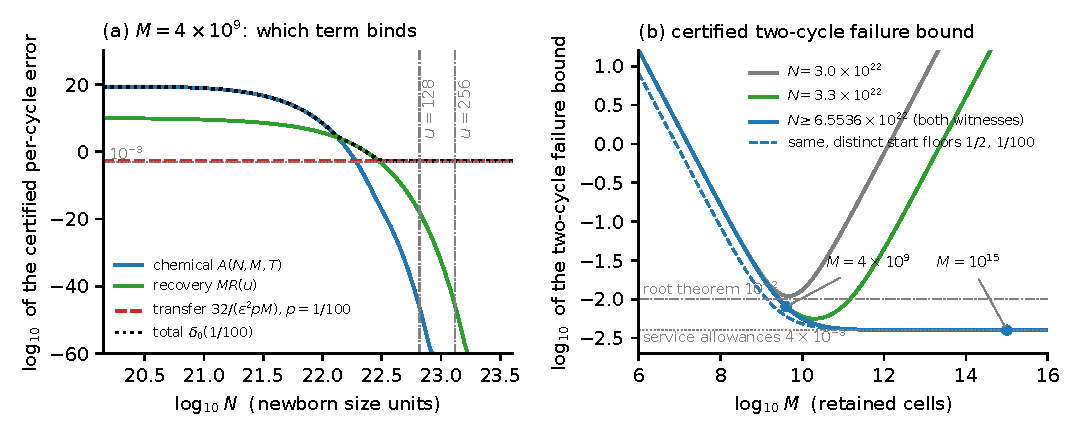
\includegraphics[width=\linewidth]{errors.pdf}
\caption{Proved bounds evaluated at 60 digits; nothing is simulated. (a) At $M=4\times10^{9}$, the per-cycle non-service error $\delta_0(1/100)$ and its three groups of terms as functions of $N$. The chemical and recovery terms are vacuous near the theorem threshold $N=1.4\times10^{20}$ ($u\approx0.27$) and fall below the transfer term only for $N$ above about $3.3\times10^{22}$, where the slowest term $2Me^{-u/2}$ drops under $10^{-4}$; beyond that the transfer term $0.002$ is the whole budget. (b) The certified two-cycle failure bound $2\delta(1/100)$ as a function of $M$. For $N\ge6.5536\times10^{22}$ it is the transfer term plus the service allowances $4\times10^{-3}$; for smaller $N$ the recovery term, proportional to $M$, lifts the plateau. Dots mark the two witnesses.}
\label{fig:errors}
\end{figure}

\paragraph{Reading of the tables and the figure.}
The constraints on scale have distinct causes. Sampling controls $M$ through $32/(\eps^2pM)$: at $M=4\times10^{9}$ this single term is $0.002$ of the certified $0.008002$ two-cycle error, and the two service allowances are the other $0.004$. Chemistry controls $N$ through $u=N\alpha a$ and the local certificate; the slowest chemical term is the recovery return $2Me^{-u/2}$, so at $M=4\times10^{9}$ the non-service error is below $0.0021$ from about $N=3.3\times10^{22}$ upward, while the theorem's hypothesis $N\ge1.4\times10^{20}$ is only where the local certificate holds. The allowed $\gamma$ fixes the batch duration $T=8/\gamma$. The uniform worst-state clock bounds make the service allowances especially conservative: the exchanged amounts of a successful trajectory are far below the quotas, which were chosen to be $1000$ times the clock-times-duration product. Reducing the sampling estimate alone cannot cure slow growth or the chemical size requirement.

\paragraph{How conservative is the transfer bound.}
Table~\ref{tab:transfer} reports an exact enumeration of the transfer sub-law for an endpoint of eight intact cells, four of each ancestry, with four cells retained. The Chebyshev bound \eqref{eq:transfer}, $32/(\eps^2\cdot\frac12\cdot4)$, exceeds one in every case, whereas the exact failure fractions are $17/35$ at tolerance $1/50$ and $1/35$ at tolerance $1/2$ for the three size-homogeneous endpoints, and $27/35$ and $13/35$ for the mixed one. Two lessons are visible: at small bottlenecks the certified bound is far from the truth, and mixed sizes among the endpoint cells genuinely raise the failure fraction, which is why the weights $m_j/(2N)$ rather than plain counts enter the argument.

\begin{table}[tb]
\centering\small
\caption{Exact conditional transfer diagnostic: eight intact endpoint cells (four per ancestry), four retained uniformly, $70$ subsets enumerated. Sizes are in $[10,20)$ with $N=10$; ``high larger'' means the four high cells have size $19$ and the low cells $10$, ``mixed'' alternates sizes within each ancestry.}
\label{tab:transfer}
\begin{tabular}{lccc}
\toprule
Endpoint & Tolerance $\eps$ & Exact failure fraction & Bound \eqref{eq:transfer}, capped\\
\midrule
Equal sizes & $1/50$ & $17/35$ & $1$\\
Equal sizes & $1/2$ & $1/35$ & $1$\\
High larger & $1/50$ & $17/35$ & $1$\\
High larger & $1/2$ & $1/35$ & $1$\\
Low larger & $1/50$ & $17/35$ & $1$\\
Low larger & $1/2$ & $1/35$ & $1$\\
Mixed sizes & $1/50$ & $27/35$ & $1$\\
Mixed sizes & $1/2$ & $13/35$ & $1$\\
\bottomrule
\end{tabular}
\end{table}

\section{Discussion}\label{sec:discussion}

\paragraph{What the theorem establishes.}
For the specified effective model, a heritable difference in resident composition produces an advantage in compartment number that survives two complete rounds of growth on a shared resource, type-blind uniform transfer of intact compartments, precursor-free recovery and refill, with explicit error for every stage and with all descendants and all retained compartments proved to be in the chemical state of their founders at every census. Three features distinguish it from a single-batch result. The retained compartments are the actual sampled ones, returned to the certified region by their own resident chemistry; the batch estimates hold for arbitrary division phases at the start, which the second cycle needs; and the phase penalty of asynchronous division is paid once at the endpoints rather than at every cycle, which is what leaves a positive count margin after two cycles.

\paragraph{What it does not establish.}
Two cycles are certified, not an unbounded sequence. The eligibility estimate $p_{k+1}\ge\frac{49}{800}p_k$ certifies a second start from a balanced one but not a third at the floors used; a longer-horizon theorem needs either a sharper sampling estimate, which is available in principle~\citep{hoeffding1963,bardenet2015}, or floors that track the actual retained counts, together with the telescoping size gain. No fixation probability, no indefinite fidelity, no emergence from arbitrary food and no autonomy of the reservoirs are claimed. The reservoirs are maintained at unit activity for a finite duration with finite gross-exchange allowances, and the size coordinate is proportional to volume by assumption. The witness sizes are astronomically large because every certificate is conservative, quadratic energies, worst-case rates over a safe box, union bounds and second moments; nothing suggests that the true failure probabilities behave like the bounds. Before an experimental application one would have to identify a calibrated size coordinate, the growth-linked concentration and its units, a well-mixed shared precursor, the growth coupling and its physical time, a classifier with error below the separation of Section~\ref{sec:consequences}, a division rule with fair per-molecule allocation, and external maintenance of the reservoirs sufficient for Table~\ref{tab:source}.

\paragraph{Relation to Moran-type and deterministic settings.}
The population of \citet{matsubara2026} keeps its size constant by random removal at each division, in the manner of the Moran process~\citep{moran1958}, and reads selection from frequency dynamics. Here the population grows from $M$ to between $2M$ and $4M$ cells within a batch, exactly $M$ are retained at transfer, and the output is a certified count-odds gain per cycle. The deterministic companion~\citep{recovery2026} proves repeated harvesting of a reversible autocatalytic reactor for arbitrary state-dependent interventions and an unbounded number of cycles, but for concentration dynamics with no finite-copy statement; the present result is a finite-copy statement for two cycles with a fixed, type-blind intervention. Combining the two, a finite-copy theorem for state-dependent interventions over many cycles, is the natural target.

\paragraph{Open questions.}
(1) A sharper sampling estimate with exponential rather than $1/M$ tails, which would reduce $M$ by many orders of magnitude and, with the eligibility floors that follow, extend the certified horizon. (2) A source estimate permitting faster growth, $\gamma$ well above $10^{-11}$, while tracking the perturbed chemical states; the batch duration $8/\gamma$ is the largest single contribution to elapsed time. (3) Recovery estimates that use the actual endpoint distribution of energies rather than the worst case $E_i\le8a$. (4) A formalized trajectory-space construction that would move Section~\ref{sec:localization} into the machine-checked part.

\paragraph{Data and code availability.}
The Lean sources, the verification receipts, the exact replay script and the figure script accompany the manuscript. \RepositoryNote

\appendix

\section{Source preparation and local certificate}\label{app:source}
With $\eps_0=10^{-5}$ and $\eta_0=10^{-4}$, the density-limit drift of the thirteen resident channels is
\begin{equation}\label{eq:drift}
f(x)=\begin{pmatrix}
6-2x_A+x_Bx_z+2\eps_0(x_B-x_A^2)\\
27+x_A-(1+x_z)x_B-\eps_0(x_B-x_A^2)\\
x_A-x_Bx_z-16x_z-4x_z^2+3x_\Hs\\
16x_z+2x_z^2-(2+\eta_0)x_\Hs
\end{pmatrix}.
\end{equation}
For a scalar $z$ put
\begin{align*}
B(z)&=\frac{60}{z+2},& K(z)&=\frac{2(1+2\eta_0)z^2-16(1-\eta_0)z}{2+\eta_0},\\
A(z)&=zB(z)+K(z),& H(z)&=\frac{16z+2z^2}{2+\eta_0}.
\end{align*}
Along the curve $x(z)=(A(z),B(z),z,H(z))$ the third and fourth coordinates of $f$ vanish identically, the second equals the residual $r(z)=27-(1+\eps_0)B(z)+K(z)+\eps_0A(z)^2$ and the first equals $-2r(z)$. The residual changes sign on each rational interval of \eqref{eq:roots}, so continuity gives $z_\lo,z_\hi$ with $f(x(z_i))=0$; only the exact endpoint signs are used and no numerical root is assumed.

For $y=(y_A,y_B,y_z,y_\Hs)$ the energies are
\[
E_i(y)=c_1y_A^2+c_2y_Ay_B+c_3y_Ay_z+c_4y_Ay_\Hs+c_5y_B^2+c_6y_By_z+c_7y_By_\Hs+c_8y_z^2+c_9y_zy_\Hs+c_{10}y_\Hs^2
\]
with the exact terminating decimals of Table~\ref{tab:coeff}. Exact positive quadratic decompositions give $\|y\|^2/200\le E_i(y)\le42\|y\|^2$.

\begin{table}[ht]
\centering\small
\caption{Coefficients of the two energies (exact decimals, hence rationals).}
\label{tab:coeff}
\begin{tabular}{crr@{\qquad}crr}
\toprule
$j$ & low & high & $j$ & low & high\\
\midrule
1 & $1.115801$ & $0.846084$ & 6 & $-4.678626$ & $-13.563286$\\
2 & $-1.227416$ & $-2.318980$ & 7 & $-6.868768$ & $-20.466056$\\
3 & $4.692094$ & $4.705706$ & 8 & $6.767757$ & $11.398763$\\
4 & $6.889770$ & $7.020116$ & 9 & $20.357612$ & $34.444552$\\
5 & $1.111499$ & $4.333988$ & 10 & $15.517433$ & $26.082111$\\
\bottomrule
\end{tabular}
\end{table}

\paragraph{Derivation of \eqref{eq:local}.}
Let $P_i$ be the symmetric matrix of $E_i$. On the box $|y_j|\le1/400$ two inequalities hold: the rational quadratic certificate $2y^{\!\top}P_iDf(s_i)y\le-\frac{84}{100}\|y\|^2$ at the root boxes, and the remainder bound $2y^{\!\top}P_i\bigl(f(s_i+y)-Df(s_i)y\bigr)\le\frac14\|y\|^2$, where the quadratic remainder of $f$ is exactly
\[
\bigl(-2\eps_0y_A^2+y_By_z,\ \ \eps_0y_A^2-y_By_z,\ \ -y_By_z-4y_z^2,\ \ 2y_z^2\bigr)
\]
and each cubic term is bounded using $|y_j|\le1/400$ and $|y_jy_k|\le\|y\|^2$. Together they give the dissipation $2y^{\!\top}P_if(s_i+y)\le-\frac{59}{100}\|y\|^2$. For a resident jump $\nu/m$ the energy increment is exactly $2y^{\!\top}P_i\nu/m+\nu^{\!\top}P_i\nu/m^2$; for growth the concentration increment is $-(x+e_z)/(m+1)$. Expanding these increments, including the falling-factorial corrections, and bounding the exponential remainders over the box gives
\[
\frac{\gen_{\gamma'}e^{N\alpha E_i}}{\alpha e^{N\alpha E_i}}\le-\frac N4\|y\|^2+2\cdot10^{8}+8\cdot10^{9}N(\gamma')^2 .
\]
The premises $N\ge1.4\times10^{20}$ and $\gamma'\le10^{-11}$ ensure $2\cdot10^{8}+8\cdot10^{9}N(\gamma')^2\le Na/672$. If $E_i\ge a/2$, use $E_i\le42\|y\|^2$ to bound the bracket by $-Na/672$; if $E_i<a/2$, use $e^{N\alpha E_i}\le e^{u/2}$ after moving $\frac u{672}e^{N\alpha E_i}$ to the left. The two cases give \eqref{eq:local} and show exactly where the scale restrictions enter. The coefficient identities and the rational remainder inequalities are verified by the source declarations listed in Appendix~\ref{app:formal}.

\section{Batch barriers}\label{app:barriers}
The unexpanded chemical bound of Proposition~\ref{prop:chem} is
\begin{align*}
A={}&e^{-8u}\Bigl(Me^u+14Me^{4u}+T\,16M\frac u{672}e^{u/2}\Bigr)\\
&+e^{-2u}\Bigl(Me^u+T\,16M\frac u{672}e^{u/2}\Bigr)+7M\Bigl(8e^{-N/(35\cdot10^{12})}\Bigr).
\end{align*}
The first barrier pays the outer crossing and the $14M$ possible daughter initializations; the second pays the division-parent crossing through the spatial observable $\exp(10^{-15}(m-2N))\exp(N\alpha E_i)$, whose size factor suppresses the daughter reset at $m=N$ and equals one at division, so that cells born at different times can be summed; the last term pays the actual complementary partitions. Expanding the exponentials gives \eqref{eq:A}.

For the size odds, with $H=B_\hi$ and $L=B_\lo$, the two logarithmic increments of $V(H,L)=\exp\bigl(\frac N{1000}[-\log H+\log L+\frac35\log(H+L)]\bigr)$ are
\begin{align*}
d_H&=\frac N{1000}\Bigl[-\log\bigl(1+\tfrac1H\bigr)+\tfrac35\log\bigl(1+\tfrac1{H+L}\bigr)\Bigr],&
d_L&=\frac N{1000}\Bigl[\log\bigl(1+\tfrac1L\bigr)+\tfrac35\log\bigl(1+\tfrac1{H+L}\bigr)\Bigr],
\end{align*}
and the sandwich \eqref{eq:sandwich} gives $Z_\hi(e^{d_H}-1)+Z_\lo(e^{d_L}-1)\le0$ for $H,L\ge N$ and $N\ge1000$, by bounding the logarithms and their exponential remainders. For the deadline, $D(H,L)=\exp\bigl(-\frac N{1000}\log\frac{H+L}{W_0}\bigr)$ on active states has generator at most $-\frac{9N\gamma}{40000}D$ before the endpoint. All barriers use Lemmas~\ref{lem:barrier}--\ref{lem:killed}; finite-domain exits are part of the failure cover, so no transition outside the domain is silently discarded.

\section{Formal statements and reproducibility}\label{app:formal}
The development is in Lean~4~\citep{demoura2021} with Mathlib~\citep{mathlib2020}, toolchain \lean{leanprover/lean4:v4.30.0}, with a frozen dependency manifest (SHA-256 \texttt{a8df0b60\ldots}). The verification bridge compiles the target and every local dependency at its current source hash, treats compiler warnings as errors, and records the axioms of each exported declaration: every declaration below uses only \lean{propext}, \lean{Classical.choice} and \lean{Quot.sound}, with no \lean{sorry} and no further axiom. The population modules are in \lean{proofs/SerialTransferSelection/} (namespace \lean{SerialTransferSelection}); the source certificates are imported from \lean{proofs/FiniteCopy/}, \lean{proofs/HeritableCompositions/} and \lean{proofs/CommonPhysicalRealization/}; the finite-kernel infrastructure from \lean{proofs/FiniteCopy/}.

\paragraph{Endpoint statements.}
The declarations \lean{smaller_newborn_instance} and \lean{original_newborn_instance} in \lean{PublicationMain.lean} state Theorem~\ref{thm:witness}: there exist stationary roots in \eqref{eq:roots}, finite clocks and quotas with the stated allowances, and a ready population of $2K$ cells with $K$ measured cells of each type, all of size $N$ and with readout equal to tag, such that the two-cycle law assigns the successful output with both measured counts positive and count log-odds gain above $2g-\log2$ probability at least $495999/500000$, respectively $497999/500000$. Both are instances of \lean{improved_serial_instance} (\lean{ImprovedInstance.lean}), which is Theorem~\ref{thm:law} with an abstract error hypothesis, itself obtained from \lean{sourceTwoCycle_newborn_probability}. The original root \lean{source_serial_transfer_c3} in \lean{Main.lean} is Remark~\ref{rem:root}. Table~\ref{tab:formal} maps the steps of this paper to modules and principal declarations.

\begin{small}
\begin{longtable}{>{\raggedright\arraybackslash}p{0.33\textwidth}>{\raggedright\arraybackslash}p{0.60\textwidth}}
\caption{Claims-to-declarations map (namespace \texttt{SerialTransferSelection} unless shown).}\label{tab:formal}\\
\toprule
Step in this paper & Modules and principal declarations\\
\midrule
\endfirsthead
\toprule
Step in this paper & Modules and principal declarations\\
\midrule
\endhead
\bottomrule
\endfoot
Resident completion, weights \eqref{eq:element}, potentials \eqref{eq:potential} & \lean{CommonPhysicalRealization/ResidentCompletion}: \lean{balanced}, \lean{thermo}, \lean{closed_resident_obstruction}, \lean{resident_projection}, \lean{growth_material}\\
Roots \eqref{eq:roots}, energies, local certificate (Lemma~\ref{lem:local}) & \lean{FiniteCopy/Source}, \lean{FiniteCopy/SourceAdapter}, \lean{FiniteCopy/QuadraticCertificates} (\lean{lowEnergy_lower}, \lean{highEnergy_lower}), \lean{HeritableCompositions/SourceAffine}\\
Finite laws, uniformization, barriers (Section~\ref{sec:tools}) & \lean{FiniteCopy/FiniteKernel}, \lean{FiniteCopy/PoissonKernel}, \lean{FiniteCopy/MarkedUniformization}; \lean{CycleLawBounds}: \lean{guardedPush_probability}, \lean{finiteLaw_joint_bind_lower}\\
Ready founders (Lemma~\ref{lem:founders}) & \lean{ReadyRegions}, \lean{InitialPopulation}, \lean{NewbornPhase}: \lean{low_ready_nonempty}, \lean{balanced_initial_newborn}\\
Conservation and caps (Lemma~\ref{lem:conservation}) & \lean{BatchConservation}: \lean{phase_batch_path_conservation}, \lean{phase_batch_population_budget}, \lean{phase_batch_division_reserve}\\
Finite batch domain and stopped model & \lean{BatchDomain}, \lean{BatchSource}, \lean{BatchSupport}: \lean{phaseStoppedModel}, \lean{phase_positive_active_domain_preserved}\\
Outer, division-parent and partition failures (Proposition~\ref{prop:chem}) & \lean{BatchOuterBoundary}, \lean{BatchOuterProbability}, \lean{BatchSpatialBoundary}, \lean{BatchSpatialProbability}, \lean{BatchPartitionEvent}, \lean{BatchPartitionProbability}, \lean{BatchChemicalProbability}: \lean{phase_global_chemical_probability}, \lean{phaseChemicalRawError}\\
Ancestral totals and size odds (Proposition~\ref{prop:odds}) & \lean{BatchAncestralBinding}, \lean{BatchAncestralPersistence}, \lean{BatchOddsProbability}: \lean{phase_global_odds_probability}\\
Deadline (Proposition~\ref{prop:deadline}) & \lean{BatchDeadlineGenerator}, \lean{BatchDeadlineProbability}: \lean{phase_global_deadline_probability}\\
Joint batch (Proposition~\ref{prop:batch}) & \lean{BatchJointEvent}, \lean{BatchJointProbability}, \lean{BatchEndpointGain}, \lean{BatchService}: \lean{phase_source_batch_joint_return}, \lean{phase_source_batch_with_service}\\
Uniform transfer law and moments (Lemmas~\ref{lem:moments}, \ref{lem:variance}) & \lean{TransferLaw}, \lean{TransferSymmetry}, \lean{TransferMoments}, \lean{TransferCovariance}, \lean{TransferVariance}: \lean{subset_pair_covariance_nonpos}, \lean{weighted_subset_variance_bound}\\
Transfer estimate (Proposition~\ref{prop:transfer}) & \lean{TransferMean}, \lean{TransferCentered}, \lean{TransferConcentration}, \lean{TransferGeometry}, \lean{TransferFrequency}, \lean{TransferPhysical}, \lean{TransferJointProbability}: \lean{source_transfer_weighted_probability}, \lean{transfer_count_frequency_floor}\\
Single-cell return (Proposition~\ref{prop:return}) & \lean{RecoverySource}, \lean{RecoveryReturn}, \lean{RecoveryExit}, \lean{RecoverySize}, \lean{RecoveryEndpoint}, \lean{RecoveryJoint}: \lean{endpoint_joint_recovery}, \lean{recoveryError}\\
Selected population return and refill (Proposition~\ref{prop:population}) & \lean{RecoveryPopulation}, \lean{RecoveryProduct}, \lean{RecoveryDock}, \lean{RecoveryRefill}, \lean{RecoveryRestart}, \lean{RecoveryService}, \lean{SelectedRecovery}: \lean{selectedRecoveryLaw_probability}, \lean{recoveredRefill_ready}\\
Capped counters and quotas (Lemmas~\ref{lem:counter}, \ref{lem:quotas}) & \lean{ServiceCounter}, \lean{ServiceJoint}, \lean{UniformClocks}: \lean{service_step_projection}, \lean{service_quota_bound}, \lean{exists_uniform_source_clocks}, \lean{exists_uniform_cycle_quotas}\\
One cycle and two cycles (Propositions~\ref{prop:cycle}, \ref{prop:two}) & \lean{CycleLaw}, \lean{CycleOutcome}, \lean{CycleTransferInputs}, \lean{CycleProbability}, \lean{TwoCycle}: \lean{sourceCycleLaw_probability}, \lean{sourceTwoCycleLaw_probability}\\
Phase identity and telescoping (Lemma~\ref{lem:phase}) & \lean{PhaseCorrection}, \lean{PopulationPhase}, \lean{NewbornPhase}: \lean{count_size_phase_identity}, \lean{mean_size_phase_bounds}, \lean{newborn_phase_corrected_cumulative_gain}, \lean{newborn_endpoint_count_gain}\\
Rational margins (Corollary~\ref{cor:fraction}, Remark~\ref{rem:root}) & \lean{ParameterMargins}, \lean{CountEnrichment}, \lean{NewbornPhase}: \lean{two_cycle_count_gain_lower}, \lean{newborn_one_cycle_rational}, \lean{newborn_two_cycle_rational}\\
Measured counts and readout & \lean{ChemicalReadout}, \lean{MeasuredCounts}: \lean{chemical_readout_matches_ancestry}, \lean{chemicalCount_eq_ancestralCount}\\
Exact error certificates (Proposition~\ref{prop:exact}) & \lean{CandidateErrors}, \lean{PostproofParameters}: \lean{candidate_nonservice_error}, \lean{smaller_nonservice_error}, \lean{original_sharp_error}, \lean{smaller_sharp_error}, \lean{exp_negative_uniform_bound}\\
Theorems~\ref{thm:law} and \ref{thm:witness} & \lean{NewbornProbability}, \lean{ImprovedInstance}, \lean{PublicationMain}: \lean{sourceTwoCycle_newborn_probability}, \lean{improved_serial_instance}, \lean{smaller_newborn_instance}, \lean{original_newborn_instance}\\
Original root (Remark~\ref{rem:root}) & \lean{NonvacuousInstance}, \lean{Main}: \lean{nonvacuous_serial_count_instance}, \lean{source_serial_transfer_c3}\\
Type neutrality, protocol certificate & \lean{ProtocolRealization}, \lean{ProtocolCertificate}: \lean{uniform_sampling_equal_mass}, \lean{sampling_ignores_tags}, \lean{refill_ignores_tags}, \lean{serial_protocol_certified}\\
Clock bounds, cutoff, accounts (Section~\ref{sec:budgets}) & \lean{AnalyticClocks}, \lean{OperationalCorollaries}, \lean{ServiceMaterial}, \lean{CycleMaterial}, \lean{DiscardAccounting}: \lean{density_clock_bound}, \lean{cell_clock_bound}, \lean{hard_budget_agreement}, \lean{explicit_quota_bound}, \lean{newborn_two_cycle_growth_stock}, \lean{two_cycle_gross_allowance}, \lean{retained_discarded_quantity}\\
Measurement error (Section~\ref{sec:consequences}) & \lean{OperationalCorollaries}: \lean{measured_fraction_difference}, \lean{observable_increase}\\
\end{longtable}
\end{small}

\paragraph{Receipts.}
The strict verification of \lean{PublicationMain.lean} (declarations \lean{smaller_newborn_instance} and \lean{original_newborn_instance}) compiled with exit code zero and empty compiler output in $75.8$~s with $184$ authenticated local dependencies; that of \lean{Main.lean} (declaration \lean{source_serial_transfer_c3}) in $63.6$~s with $178$ dependencies. Source SHA-256 of \lean{PublicationMain.lean}:
\begin{center}\footnotesize\ttfamily
7e2d530590d2ea3927ddaa19d5869c1e671b34728c0bc963272061bd15efb26c
\end{center}
and of \lean{Main.lean}:
\begin{center}\footnotesize\ttfamily
3e7d4c875601ca37f90beb892c77b0e5a1609802cffac0b8bda892d7b23bdf05 .
\end{center}
Within the development, verification is reproduced from the repository root by
\begin{quote}\scriptsize\ttfamily\raggedright
python scripts/verify\_proof.py proofs/SerialTransferSelection/PublicationMain.lean \textbackslash\\
\hspace*{2em}--timeout 600 --declaration SerialTransferSelection.smaller\_newborn\_instance \textbackslash\\
\hspace*{2em}--declaration SerialTransferSelection.original\_newborn\_instance
\end{quote}
which pins the working directory \lean{mathlib4_project/} and the toolchain and rejects warnings, admitted proofs and nonzero exits. Hashes document the correspondence between receipts and sources; they are not mathematical evidence by themselves, and counts of receipts are reproducibility metadata, not counts of results.

\paragraph{Formal scope.}
Lean verifies: the finite marked laws and their Poissonized kernels; the guarded push and conditional composition; the resident completion identities; the roots, energies and local certificate; the batch conservation and caps; the outer, division-parent, partition, size-odds and deadline bounds and their union; the uniform transfer law, its moments, the variance bound, the concentration and geometry statements; the single-cell and selected-population recovery bounds, docking and refill; the capped counters, quota bounds and existence of clocks and quotas; the one- and two-cycle laws and their bounds; the phase identity, the newborn phase and the count conversion; the readout identification; the exact rational error certificates; Theorems~\ref{thm:law} and \ref{thm:witness}, Corollary~\ref{cor:fraction} (rational thresholds) and the original root; the protocol certificate; the density and cell clock bounds, the explicit quota inequality, the finite-word cutoff agreement, the $12NM$ stock bound, the discard identity and the two-cycle gross allowance; and the measurement-error implication. Conventional: the continuous-time reading of Section~\ref{sec:localization}; the population summation from the verified per-cell clock bound to \eqref{eq:clocks}; the lifting of the finite-word cutoff to the marked-clock interpretation; the decimal values of the exact thresholds; the interpretations of Section~\ref{sec:discussion}. Numerical, not proof: Table~\ref{tab:terms}, the evaluated rows of Table~\ref{tab:witness}, Figure~\ref{fig:errors}, and the exact enumeration of Table~\ref{tab:transfer}, which is a diagnostic of a sub-law and not part of the theorem.

\bibliographystyle{plainnat}
\bibliography{refs}

\end{document}
